\chapter{Kleinste Zahl in einem Array finden}

\begin{enumerate}
  \item Zuerst initialisieren wir den Wert des gesuchten Minimums auf das erste
  Element des Arrays. Im nächsten Schritt durchlaufen wir das Array Eintrag für
  Eintrag in einer for-Schleife. Falls der Wert des aktuellen Eintrags kleiner
  ist als das bisher gefundene Minimum, ersetzen wir den Wert des Minimums
  durch den Wert des Eintrags.

  \textit{Hinweis}: für die generische und damit automatische Ermittlung der
  Größe des Arrays verwenden wir hier den Ausdruck:

\noindent\mintinline{c}{int arraySize = sizeof(myArray) / sizeof(int);}

\begin{minted}{c}
#include <stdio.h>

int main(void) {
    int myArray[] = {4, 2, 9, 24, 4, 8, 5, 24};
    int arraySize = sizeof(myArray) / sizeof(int);

    int min;

    min = myArray[0];
    for (int i = 0; i < arraySize; i++) {
        if (myArray[i] < min) {
            min = myArray[i];
        }
    }

    printf("Kleinstes Element: %d\n", min);
}
\end{minted}

  \item In diesem Fall erstellen wir eine Funktion, die zwei Eingabeparameter
  besitzt: ein int-Array und einmal die Größe des Arrays. Der Funktionssignatur
  kann das Array in zwei gleichbedeutenden Formen entgegennehmen: entweder als
  \mintinline{c}{int array[]} oder als \mintinline{c}{int *array}. Die Größe
  des Arrays muss der Funktion übergeben werden, da sie diese ansonsten nicht
  erkennen kann.

\begin{minted}{c}
#include <stdio.h>

int find_min(int array[], int size) {
    int min = array[0];
    for (int i = 1; i < size; i++) {
        if (array[i] < min) {
            min = array[i];
        }
    }
    return min;
}

int main(void) {
    int myArray[] = {4, 2, 9, 24, 4, 8, 5, 24};
    int arraySize = sizeof(myArray) / sizeof(int);

    int min = find_min(myArray, arraySize);

    printf("Kleinstes Element: %d\n", min);
}
\end{minted}

\end{enumerate}



\chapter{Häufigkeiten eines Werts in einem Array zählen}

\begin{enumerate}
\item Zuerst legen wir eine Variable \mintinline{c}{count} an, die wir mit dem
Wert 0 initialisieren. Im nächsten Schritt durchlaufen wir das Array Eintrag
für Eintrag in einer for-Schleife. Falls der Wert des aktuellen Eintrags dem
gesuchten Wert entspricht, erhöhen wir den Zähler count um Eins.

\textit{Hinweis}: für die generische und damit automatische Ermittlung der
Größe des Arrays verwenden wir hier den Ausdruck:

\noindent\mintinline{c}{int arraySize = sizeof(myArray) / sizeof(int);}

\begin{minted}{c}
#include <stdio.h>

int main(void) {
    int myArray[] = {4, 2, 9, 24, 4, 8, 5, 24};
    int to_find = 4;
    int arraySize = sizeof(myArray) / sizeof(int);

    int count = 0;
    for (int i = 0; i < arraySize; i++) {
        if (myArray[i] == to_find)
            count++;
    }

    printf("Anzahl in Array: %d\n", count);
}
\end{minted}

\item In diesem Fall erstellen wir eine Funktion, die drei Eingabeparameter
besitzt: ein int-Array, dann die Größe des Arrays und schließlich noch die
Zahl, nach der gesucht werden soll.

Auch hier ist es so, dass wir die Größe des Arrays an die Funktion übergeben
müssen, da sie sonst innerhalb der Funktion nicht ermittelt werden kann.

\begin{minted}{c}
#include <stdio.h>

int occurrences(int array[], int size, int to_find) {
    int count = 0;

    for (int i = 0; i < size; i++) {
        if (array[i] == to_find)
            count++;
    }
    return count;
}

int main(void) {
    int myArray[] = {4, 2, 9, 24, 4, 8, 5, 24};
    int to_find = 4;
    int arraySize = sizeof(myArray) / sizeof(int);

    int count = occurrences(myArray, arraySize, to_find);

    printf("Anzahl in Array: %d\n", count);
}
\end{minted}

\end{enumerate}



\chapter{Reihenfolge eines Arrays umkehren}

\begin{enumerate}
    \item Um die Elemente eines Arrays umzukehren, müssen wir eine typische
    \mintinline{c}{swap}-Operation realisieren. Dazu brauchen wir eine
    temporäre Variable (\mintinline{c}{temp}), in der wir das auszutauschende
    Element zwischenspeichern.

    Beim Durchlaufen des Arrays vertauschen wir schrittweise die Elemente der
    ersten Hälfte in aufsteigender Form mit den Elementen der zweiten Hälfte in
    absteigender Form.

    Beachten Sie hier den Ausdruck:

    \noindent\mintinline{c}{myArray[arraySize - i - 1]}

    Da Arrays vom Index 0 beginnend adressiert werden und nur bis zum Index
    \textit{Größe minus 1}, müssen wir die Zahl 1 bei der Berechnung abziehen.

    Beachten Sie, dass die Berechnung sowohl für eine gerade als auch eine
    ungerade Anzahl an Elementen funktioniert. Das liegt an der Art und Weise,
    wie in C eine Ganzzahl-Division durchgeführt wird, bei der das Ergebnis auf
    die nächstkleinere Zahl gerundet wird (also nicht mathematisch gerundet).

    \textit{Hinweis}: für die generische und damit automatische Ermittlung der
    Größe des Arrays verwenden wir hier den Ausdruck:

    \noindent\mintinline{c}{int arraySize = sizeof(myArray) / sizeof(int);}

\begin{minted}{c}
#include <stdio.h>

int main(void) {
    int myArray[] = {4, 2, 9, 24, 4, 8, 5, 24};
    int arraySize = sizeof(myArray) / sizeof(int);
    int temp = 0;

    for (int i = 0; i < (arraySize / 2); i++) {
        temp = myArray[i];
        myArray[i] = myArray[arraySize - i - 1];
        myArray[arraySize - i - 1] = temp;
    }

    printf("Umgekehrte Reihenfolge:\n");
    for (int i = 0; i < arraySize; i++) {
        printf("myArray[%d] = %d\n", i, myArray[i]);
    }
}
\end{minted}

\item Bei der Auslagerung der Berechnung in eine eigenständige Funktion müssen
enstprechend das Array und die Größe an die Funktion übergeben werden. Der
Rückgabewert ist \mintinline{c}{void}, da die Funktion die Elemente im Array
direkt umkehrt und daher keinen Wert an den Aufrufer zurückliefern muss.

\begin{minted}{c}
#include <stdio.h>

void reverse(int array[], int size) {
    int temp = 0;

    for (int i = 0; i < (size / 2); i++) {
        temp = array[i];
        array[i] = array[size - i - 1];
        array[size - i - 1] = temp;
    }
}

int main(void) {
    int myArray[] = {4, 2, 9, 24, 4, 8, 5, 24};
    int arraySize = sizeof(myArray) / sizeof(int);

    reverse(myArray, arraySize);

    printf("Umgekehrte Reihenfolge:\n");
    for (int i = 0; i < arraySize; i++) {
        printf("myArray[%d] = %d\n", i, myArray[i]);
    }
}
\end{minted}

\end{enumerate}



\chapter{Barcode-Prüfziffer berechnen}

Die Funktion \mintinline{c}{convertStringToArray()} nimmt einen String und ein
Array als Argumente und konvertiert den String in ein Integer-Array. Zunächst
wird überprüft, ob der String genau 12 Zeichen lang ist. Falls nicht, gibt die
Funktion eine Fehlermeldung aus und kehrt mit einem Fehlercode (1) zurück.

Anschließend wird geprüft, ob jedes Zeichen im String eine Ziffer ist, indem die
Funktion \mintinline{c}{isdigit()} verwendet wird. Wenn eine Nicht-Ziffer
gefunden wird, gibt die Funktion erneut eine Fehlermeldung aus und kehrt mit
einem Fehlercode (2) zurück.

Sind alle Zeichen Ziffern, konvertiert die Funktion jedes Zeichen in seine
entsprechende Zahl, indem sie den ASCII-Wert von \mintinline{c}{'0'} vom Zeichen
subtrahiert, und speichert die Ziffern im Array. Abschließend wird der Erfolg
durch Rückgabe von 0 signalisiert.

\begin{minted}{c}
int convertStringToArray(const char *str, int barcode[]) {
    // Überprüfen, ob der String genau 12 Ziffern enthält
    if (strlen(str) != BARCODE_LENGTH) {
        printf("Fehler: String muss 12 Zeichen lang sein.\n");
        return 1;  // Fehlercode zurückgeben
    }

    // Überprüfen, ob der String nur Ziffern enthält
    for (int i = 0; i < 12; i++) {
        if (!isdigit(str[i])) {
            printf("Fehler: String darf nur Ziffern enthalten.\n");
            return 2;  // Fehlercode zurückgeben
        }
    }

    // Konvertieren der Zeichen in Integer
    for (int i = 0; i < 12; i++) {
        // ASCII-Wert von '0' subtrahieren,
        // um die Ziffer zu erhalten
        barcode[i] = str[i] - '0';
    }

    return 0;  // Erfolgscode zurückgeben
}
\end{minted}

Die Funktion \mintinline{c}{barcodeCheckDigit()} berechnet die Prüfziffer eines
EAN-Barcodes basierend auf einem gegebenen Integer-Array und dessen Länge.
Hierzu wird der Algorithmus aus der Aufgabenstellung entsprechend angewendet.
Die Funktion gibt schließlich die berechnete Prüfziffer zurück.

\begin{minted}{c}
int barcodeCheckDigit(int barcode[], int barcodeLength) {
    int oddSum = 0, evenSum = 0, totalSum = 0;
    int checkDigit = 0;

    // Berechne die Summe der ungeraden und geraden Ziffern
    for (int i = 0; i < barcodeLength; i++) {
        if (i % 2 == 0) {
            // Ungerade Positionen (Index 0, 2, 4,...)
            oddSum += barcode[i];
        } else {
            // Gerade Positionen (Index 1, 3, 5,...)
            evenSum += barcode[i];
        }
    }

    // Multipliziere die Summe der geraden Positionen mit 3
    // und addiere diese Summe mit der Summe der ungeraden Zahlen
    totalSum = oddSum + (evenSum * 3);

    // Berechne die Prüfziffer
    checkDigit = 10 - (totalSum % 10);
    if (checkDigit == 10) {
        checkDigit = 0;
    }

    return checkDigit;
}
\end{minted}




\chapter{Text in Leetspeak umwandeln}

Die Funktion \mintinline{c}{getLeetChar()} soll ein einzelnes Zeichen als
Argument erhalten und ein einzelnes Zeichen an den Aufrufer zurückgeben. Die
entsprechende Funktionssignatur lautet entsprechend:

\mintinline{c}{char getLeetChar(char c)}

Bei der Konvertierung muss überprüft werden, ob für das übergebene Zeichen ein
alternatives "Leetspeak"-Zeichen existiert. Falls dies der Fall ist, wird das
Zeichen durch das entsprechende Leetspeak-Zeichen ersetzt. Hierfür bietet sich
eine \mintinline{c}{switch-case}-Anweisung an.

Es ist dabei wichtig zu beachten, dass sowohl Groß- als auch Kleinschreibung
berücksichtigt werden müssen und die \mintinline{c}{break}-Anweisungen nicht
vergessen werden dürfen.

\begin{minted}{c}
char getLeetChar(char c) {
    switch (c) {
    case 'A':
    case 'a':
        c = '4';
        break;
    case 'B':
    case 'b':
        c = '8';
        break;
    case 'E':
    case 'e':
        c = '3';
        break;
    case 'G':
    case 'g':
        c = '6';
        break;
    case 'H':
    case 'h':
        c = '#';
        break;
    case 'I':
    case 'i':
        c = '1';
        break;
    case 'O':
    case 'o':
        c = '0';
        break;
    case 'S':
    case 's':
        c = '$';
        break;
    case 'T':
    case 't':
        c = '7';
        break;
    case 'Z':
    case 'z':
        c = '2';
        break;
    default:
        break;
    }

    return c;
}
\end{minted}

Die Funktion \mintinline{c}{leetspeak()} nimmt einen String als Argument und
wandelt ihn mithilfe der Funktion \mintinline{c}{getLeetChar()} in Leetspeak um.
Dabei wird jedes Zeichen des Strings einzeln durchlaufen und durch
\mintinline{c}{getLeetChar()} überprüft, ob eine Ersetzung erforderlich ist.

Die Funktionsweise basiert auf einer Schleife, die den String Zeichen für
Zeichen verarbeitet, bis das Nullterminierungszeichen \mintinline{c}{'\0'}
erreicht wird. Jedes Zeichen wird an die \mintinline{c}{getLeetChar()}-Funktion
übergeben, und der Rückgabewert dieser Funktion ersetzt das jeweilige Zeichen im
Original-String. Auf diese Weise wird der gesamte String in Leetspeak
konvertiert.

\begin{minted}{c}
void leetspeak(char *str) {
    for (int i = 0; str[i] != '\0'; i++) {
        str[i] = getLeetChar(str[i]);
    }
}
\end{minted}










\chapter{Überprüfen, ob ein String ein Palindrom ist}

Die \mintinline{c}{isPalindrome()}-Funktion bekommt einen String übergeben und
gibt einen Booleschen Wert (\mintinline{c}{true} oder \mintinline{c}{false}) an
den Aufrufer zurück. Dafür haben wir den Header \mintinline{c}{stdbool.h}
eingebunden.

Zuerst ermitteln wir die Länge und die Mitte des Strings mithilfe der
\mintinline{c}{strlen()}-Funktion aus dem \mintinline{c}{string.h}-Header. Das
Ergebnis ist der Index, der die Mitte des Strings markiert. Bei der Überprüfung
auf ein Palindrom wird dieser Wert verwendet, um nur bis zur Mitte des Strings
zu iterieren, da die zweite Hälfte des Strings spiegelbildlich zur ersten Hälfte
sein sollte, wenn es sich um ein Palindrom handelt.

In der Funktion wird eine for-Schleife verwendet, die bis zur Mitte des Strings
läuft. Jedes Zeichen der ersten Stringhälfte wird mit dem korrespondierenden
Zeichen von hinten verglichen. Da die Groß-/Kleinschreibung keine Rolle spielen
soll, verwenden wir die \mintinline{c}{tolower()}-Funktion aus dem
\mintinline{c}{ctype.h}-Header.

Stimmen zwei miteinander verglichenen Zeichen nicht überein, wird die Funktion
direkt beendet und der Wert \mintinline{c}{false} an den Aufrufer zurückgegeben.
Falls bis zum Ende des Schleifendurchlaufs keine Unstimmigkeiten aufgetreten
sind, gibt die Funktion \mintinline{c}{true} zurück.

\begin{minted}{c}
#include <stdio.h>
#include <stdbool.h>
#include <string.h> // für strlen()
#include <ctype.h>  // für tolower()

bool isPalindrome(char string[]) {
    int len = (int)strlen(string);
    int middle = len / 2;

    for (int i = 0; i < middle; i++) {
        if (tolower(string[i]) != tolower(string[len - i - 1]))
            return false;
    }
    return true;
}
\end{minted}



\chapter{Strings unter Verwendung dynamischer Speicherzuweisung verbinden}

Da die Funktion \mintinline{c}{stringAppend()} dynamisch Speicher auf dem Heap
für den neuen String reservieren soll, müssen zunächst die Längen der beiden
übergebenen Strings mithilfe der \mintinline{c}{strlen()}-Funktion ermittelt
werden. Da \mintinline{c}{strlen()} das abschließende Nullendezeichen eines
Strings nicht in seiner Längenberechnung berücksichtigt, wird in der Berechnung
der Gesamtlänge ein zusätzliches Byte für dieses Endezeichen eingerechnet:

\mintinline{c}{size_t lengthTotal = length1 + length2 + 1;}

Als nächstes nutzen wir die \mintinline{c}{malloc()}-Funktion aus dem
\mintinline{c}{stdlib.h}-Header, um den Speicher dynamisch auf dem Heap zu
reservieren.

Daraufhin kopieren wir zeichenweise die Zeichen aus den übergebenen Strings in
den neu allokierten Speicherbereich; zuerst für den ersten String, dann für den
zweiten. Beim zweiten Kopiervorgang müssen wir darauf achten, dass wir ab dem
richtigen Index anfangen, die Zeichen zu kopieren.

Abschließend dürfen wir nicht vergessen, dass Nullendezeichen an den neuen
String anzuhängen, um den neuen String korrekt zu terminieren und den Pointer
auf den Speicherbereich des neuen Strings an den Aufrufer zurückliefern.

Bei einer Lösung wie dieser ist es wichtig, daran zu denken, dass der Speicher
für diesen neuen String später mit \mintinline{c}{free()} freigegeben wird, um
Speicherlecks zu vermeiden.

\begin{minted}{c}
char *stringAppend(char *firstString, char *secondString) {
    size_t length1 = strlen(firstString);
    size_t length2 = strlen(secondString);
    size_t lengthTotal = length1 + length2 + 1;

    char *concatenatedString = malloc(lengthTotal * sizeof(char));

    for (size_t i = 0; i < length1; i++)
        concatenatedString[i] = firstString[i];

    for (size_t i = 0; i < length2; i++)
        concatenatedString[length1 + i] = secondString[i];

    concatenatedString[lengthTotal - 1] = '\0';

    return concatenatedString;
}
\end{minted}





\chapter{Häufigste vorkommende Zeichen in einem String finden}

Um das am häufigsten vorkommende Zeichen in einem String zu ermitteln, ist es
notwendig, den String mehrfach zu durchlaufen. Dies erfordert zwei ineinander
verschachtelte Schleifen: In der äußeren Schleife wird jeweils ein Zeichen aus
dem String entnommen und in der Variablen \mintinline{c}{currentChar}
gespeichert. Anschließend zählen wir in der inneren Schleife die Häufigkeit
dieses Zeichens im gesamten String, wofür die Variable
\mintinline{c}{currentOccurrence} verwendet wird. Hierfür reicht es, wenn die
innere Schleife von der aktuellen Position der äußeren Schleife bis zum Ende des
Strings läuft.

Wichtig ist, dass wir bei jedem neuen Durchlauf der äußeren Schleife die
Variablen \mintinline{c}{currentChar} und \mintinline{c}{currentOccurrence} neu
initialisieren. Falls das aktuell betrachtete Zeichen
(\mintinline{c}{currentChar}) identisch mit dem bis dahin am häufigsten
gefundenen Zeichen (\mintinline{c}{maxChar}) ist, können wir dieses Zeichen
überspringen und direkt zum nächsten fortschreiten, um redundante Zählungen zu
vermeiden.

In der inneren Schleife vergleichen wir jedes Zeichen des Strings mit
\mintinline{c}{currentChar}. Stimmen sie überein, erhöhen wir
\mintinline{c}{currentOccurrence}. Nach Abschluss der inneren Schleife prüfen
wir, ob \mintinline{c}{currentOccurrence} größer als die bisherige maximale
Häufigkeit (\mintinline{c}{maxOccurrence}) ist. Ist dies der Fall, aktualisieren
wir die Variablen \mintinline{c}{maxChar} und \mintinline{c}{maxOccurrence}
entsprechend.

\begin{minted}{c}
void printMaxChars(char *string) {
    size_t length = strlen(string);
    char maxChar = '\0';
    char currentChar;
    int maxOccurrence = 0;
    int currentOccurrence = 0;

    for (size_t i = 0; i < length; i++) {
        currentChar = string[i];
        currentOccurrence = 0;
        if (currentChar == maxChar)
            continue;
        for (size_t j = i; j < length; j++) {
            if (string[j] == currentChar)
                currentOccurrence++;
        }
        if (currentOccurrence > maxOccurrence) {
            maxOccurrence = currentOccurrence;
            maxChar = currentChar;
        }
    }

    printf("Zeichen %c kommt %d mal vor.\n", maxChar, maxOccurrence);
}
\end{minted}





\chapter{Anzahl Wörter in einem String zählen}

Bei dieser Aufgabenstellung spielen zwei Dinge eine wesentliche Rolle: es ist
wichtig zu verstehen, woran wir erkennen, was ein Wort ausmacht; zum anderen
müssen wir eine Strategie entwickeln, um durch den String zu laufen, um nach
Wörtern zu suchen.

Direkt vor einem eigenständigen Wort muss ein Leerraumzeichen stehen, denn wenn
wir nach dem Wort "Mutter" suchen, soll "Tagesmutter" nicht mitgezählt werden.
Die einzige Ausnahme dieser Regel wäre das allererste Zeichen im String.
Außerdem darf das Zeichen hinter dem gesuchten Wort wiederum kein alphabetisches
Zeichen sein, denn wenn wir nach dem Wort "Mutter" suchen, sollte "Muttertag"
wiederum nicht mitgezählt werden.

Bezüglich der Strategie müssen wir auf jeden Fall zeichenweise durch den
gesamten String laufen. Das tun wir in Zeile 11 mittels der while-Schleife, die
solange läuft, bis das nachfolgende Zeichen dem String-Endezeichen entspricht.
Für den aktuell zu untersuchenden Index des Strings verwenden wir die Variable
\mintinline{c}{stringPos}, die entsprechend sukzessive erhöht werden muss.

Jetzt wenden wir die Suchkriterien an: zuerst prüfen wir, ob das Zeichen am
aktuell verwendeten Index überhaupt ein alphabetisches Zeichen ist. Falls nicht,
können wir direkt den Index erhöhen und den nächsten Schleifendurchlauf starten
(Zeilen 14-17).

Hatten wir am aktuellen Index ein alphabetisches Zeichen, dann geht es darum, zu
prüfen, ob das Zeichen davor ein Leerraumzeichen war (mit der Ausnahme des
allerersten Zeichens im String) (Zeilen 19-22).

War auch diese Prüfung erfolgreich, stehen wir offensichtlich an einem Wortanfang
und es geht darum die nächsten Zeichen des Strings mit denen unseres Suchworts
zu vergleichen.

Hierfür verwenden wir eine for-Schleife, die maximal so viele Durchläufe
durchläuft, wie das Suchwort Zeichen enthält (\mintinline{c}{lenWord}). Wir
vergleichen jetzt jedes Zeichen des Suchworts am Index \mintinline{c}{wordPos}
mit dem Zeichen des Strings am Index \mintinline{c}{stringPos}. Da wir die
Groß-/Kleinschreibung nicht berücksichtigen wollen, wenden wir auf beide Zeichen
die \mintinline{c}{tolower()}-Funktion an.

\begin{figure}[htb!]
    \begin{tikzpicture}[font=\ttfamily, node distance=0mm, every node/.style={minimum size=1cm, align=center}]
        % Erste Zeile von Quadraten
        \node[draw] (s1) {F};
        \node[draw, right=of s1] (s2) {i};
        \node[draw, right=of s2] (s3) {s};
        \node[draw, right=of s3] (s4) {c};
        \node[draw, right=of s4] (s5) {h};
        \node[draw, right=of s5] (s6) {e};
        \node[draw, right=of s6] (s7) {r};
        \node[draw, right=of s7] (s8) {s};
        \node[draw, right=of s8] (s9) {};
        \node[draw, right=of s9] (s10) {F};
        \node[draw, right=of s10] (s11) {r};
        \node[draw, right=of s11] (s12) {i};
        % Spezialbox mit gestrichelten Linien und ohne rechte Linie
        \node[right=of s12, minimum height=1cm, minimum width=1cm, align=center] (s13) {$\cdots$};
        \draw[dashed] (s13.north west) -- (s13.north east);
        \draw[dashed] (s13.south west) -- (s13.south east);

        % Beschriftung für die erste Zeile
        \node[above=0.3cm of s1, minimum size=0, draw=none] {stringPos};
        \draw[-{Latex[length=2mm,width=2mm]}] ([yshift=0.35cm]s1.north) -- (s1.north);

        % Beschriftung links von der ersten Zeile
        \node[left=of s1, minimum size=0, draw=none] {string};

        % Zweite Zeile von Quadraten
        \node[draw, below=1cm of s1] (w1) {F};
        \node[draw, right=of w1] (w2) {i};
        \node[draw, right=of w2] (w3) {s};
        \node[draw, right=of w3] (w4) {c};
        \node[draw, right=of w4] (w5) {h};
        \node[draw, right=of w5] (w6) {e};

        % Beschriftung für die zweite Zeile
        \node[above=0.3cm of w1, minimum size=0, draw=none] {wordPos};
        \draw[-{Latex[length=2mm,width=2mm]}] ([yshift=0.35cm]w1.north) -- (w1.north);

        % Beschriftung links von der zweiten Zeile
        \node[left=of w1, minimum size=0, draw=none] {word};
    \end{tikzpicture}
\end{figure}

Falls die beiden Zeichen nicht übereinstimmen, entspricht das gerade untersuchte
Wort im String nicht unserem Suchwort. Wir setzen daher unseren booleschen Wert
\mintinline{c}{wordFound} auf \mintinline{c}{false} und brechen aus der inneren
Schleife aus.

Andernfalls müssten alle Zeichen des untersuchten Worts dem unseres Suchtworts
entsprochen haben. Dann geht es darum, zu prüfen, ob das untersuchte Wort auch
abgeschlossen ist, wofür hinter dem untersuchten Wort ein Leerraumzeichen stehen
müsste. Dafür prüfen wir in Zeile 22, ob an der nun folgenden Stelle ein
alphabetisches Zeichen steht.

Sollte dies zutreffen, so haben wir das Suchwort leider nicht gefunden und
müssen einen Schritt weiter im Index und die Suche erneut mit einem neuen
Schleifendurchlauf starten.

Andernfalls haben wir das Suchwort tatsächlich gefunden und können jetzt den
Zähler \mintinline{c}{wordCount} um Eins erhöhen (Zeile 37-38).

Abschließend müssen wir für die while-Schleife noch dafür sorgen, dass der Index
für den nächsten Schleifendurchlauf um Eins erhöht wird.

\begin{minted}[linenos]{c}
#include <stdio.h>
#include <string.h> // für strlen()
#include <ctype.h>  // für tolower() und isalpha()
#include <stdbool.h>

int countWords(char string[], char word[]) {
    int lenWord = (int)strlen(word);
    int wordCount = 0;
    int stringPos = 0;

    while (string[stringPos + 1] != '\0') {
        bool validWord = true;

        if (!isalpha(string[stringPos])) {
            stringPos++;
            continue;
        }

        if (stringPos != 0 && string[stringPos - 1] != ' ') {
            stringPos++;
            continue;
        }

        for (int wordPos = 0; wordPos < lenWord; wordPos++) {
            if (tolower(string[stringPos]) != tolower(word[wordPos])) {
                validWord = false;
                break;
            }
            stringPos++;
        }

        if (isalpha(string[stringPos])) {
            stringPos++;
            continue;
        }

        if (validWord)
            wordCount++;

        stringPos++;
    }

    return wordCount;
}
\end{minted}






\chapter{Durchschnitt von Gruppen von Zahlen in einer Datei finden}

Im Folgenden werden Ihnen zwei mögliche Lösungen vorgestellt. Eine, bei der wir
die Zeile komplett in einen Puffer einlesen und dann mit der
\mintinline{c}{strtok()}-Funktion in einzelne "\textit{Tokens}" zerlegen; und
eine, bei der wir keinen separaten Puffer anlegen und direkt mit der
\mintinline{c}{fscanf()}-Funktion Ganzzahlen aus der Datei einlesen.

\section*{Variante mit \texttt{strtok}}

Um die Gruppen an Zahlen aus der Datei auszulesen, müssen wir zuerst die Datei
lesend mittels \mintinline{c}{fopen()} öffnen und prüfen, ob das Öffnen
erfolgreich war. Darauffolgend können wir eine Zeile aus der Datei einlesen.
Falls wir davon ausgehen, dass es nur eine Zeile ist und diese nicht länger als
maximal 256 Zeichen ist, reicht ein einzelner Aufruf der
\mintinline{c}{fgets()}-Funktion, um die Zeile in den temporären Puffer
\mintinline{c}{buf} einzulesen.

Jetzt können wir den Inhalt der Zeile interpretieren. Wenn wir wissen, dass die
einzelnen Zahlen mittels Leerzeichen voneinander getrennt sind, können wir die
\mintinline{c}{strtok()}-Funktion aus dem \mintinline{c}{string.h}-Header
verwenden, um immer einzelne Tokens einzulesen.

Der erste Aufruf von \mintinline{c}{strtok()} muss auf den Beginn der Zeile
zeigen. Das Token (also hier die erste Zahl) kann dann durch den Pointer
\mintinline{c}{p} ausgelesen und mittels der \mintinline{c}{atoi()}-Funktion in
eine Ganzzahl umgewandelt werden. Folgende Aufrufe von \mintinline{c}{strtok()}
müssen dann jedoch immer als erstes Argument \mintinline{c}{NULL} nutzen, um
weiter im String voranzuschreiten.

Wenn wir wissen, wie viele Zahlen eine Gruppe umfasst, können wir in einer
darauffolgenden for-Schleife entsprechend viele Zahlen einlesen, aufsummieren
und schließlich den Durchschnitt berechnen.

Die größte Schwierigkeit könnte darin bestehen, dies kontinuierlich so lange für
Gruppen von Zahlen durchzuführen, bis das Zeilenende erreicht ist. Wenn wir
\mintinline{c}{strtok()} einsetzen, können wir uns zunutze machen, dass die
Funktion am Zeilenende \mintinline{c}{NULL} zurückliefert und wir
dementsprechend den Aufruf in einer \mintinline{c}{while}-Schleife anwenden
können.

\begin{minted}{c}
#include <stdio.h>
#include <string.h> // für strtok()
#include <stdlib.h> // für atoi()

int main(void) {
    char *filename = "08_group_of_numbers.txt";
    FILE *fp = fopen(filename, "r");
    if (fp == NULL) {
        printf("Fehler beim Öffnen der Datei\n");
        return -1;
    }

    char buf[256];
    if (fgets(buf, 255, fp) == NULL) {
        printf("Fehler beim Einlesen der Zeile");
        return -2;
    }

    int groupLength;
    int groupSum;
    double groupAverage;
    char *p;
    p = strtok(buf, " ");
    while (p != NULL) {
        groupLength = atoi(p);
        groupSum = 0;
        groupAverage = 0;
        for (int i = 0; i < groupLength; i++) {
            p = strtok(NULL, " ");
            if (p == NULL) {
                printf("Unerwartetes Ende der Zeile\n");
                return -3;
            }
            groupSum += atoi(p);
        }
        groupAverage = (double)groupSum / groupLength;
        printf("Gruppe mit %d Elementen: %.2lf\n", groupLength, groupAverage);

        // Bereite die nächste Gruppe vor
        p = strtok(NULL, " ");
    }

    fclose(fp);
}
\end{minted}

Statt eine statische Puffergröße von 256 Zeichen festzulegen, könnten wir zuerst
auslesen, wie lang die Zeile in der Datei ist und daraufhin entsprechend viel
dynamischen Speicher allokieren:

\begin{minted}{c}
// Ermittle die Länge der Zeile
fseek(fp, 0, SEEK_END);
long length = ftell(fp);
fseek(fp, 0, SEEK_SET);

// Allokiere Speicher für die Zeile
char *buf = (char *)malloc((unsigned long)length + 1);
if (buf == NULL) {
    printf("Speicherzuweisungsfehler\n");
    fclose(fp);
    return -1;
}

if (fgets(buf, (int)length + 1, fp) == NULL) {
    printf("Fehler beim Einlesen der Zeile\n");
    free(buf);
    fclose(fp);
    return -2;
}

// [...]

free(buf);
fclose(fp);
\end{minted}

\section*{Variante mit \texttt{fscanf}}

Die alternative Lösung nutzt die \mintinline{c}{fscanf()}-Funktion, um die
Zahlen direkt aus der Datei zu lesen. Zuerst wird \mintinline{c}{fscanf()} in
einer while-Schleife verwendet, um die Länge jeder Gruppe einzulesen. Innerhalb
dieser Schleife wird eine for-Schleife mit einer Anzahl von Durchläufen gleich
der Gruppenlänge verwendet. In jedem Durchlauf dieser for-Schleife rufen wir
\mintinline{c}{fscanf()} erneut auf, um den nächsten Ganzzahlwert aus der Datei
einzulesen. Bei jedem Aufruf von \mintinline{c}{fscanf()} bewegt sich der
interne "\textit{File Position Pointer}" weiter, sodass kontinuierlich durch die
Datei gelesen wird. Dieser Ansatz eliminiert die Notwendigkeit, die gesamte
Zeile zuerst in einen Puffer zu lesen und dann zu zerlegen

\begin{minted}{c}
#include <stdio.h>
#include <stdlib.h> // für malloc und free

int main(void) {
    char *filename = "08_group_of_numbers.txt";
    FILE *fp = fopen(filename, "r");
    if (fp == NULL) {
        printf("Fehler beim Öffnen der Datei\n");
        return -1;
    }

    int groupLength;
    int number;
    int groupSum;
    double groupAverage;

    while (fscanf(fp, "%d", &groupLength) == 1) {
        groupSum = 0;
        groupAverage = 0.0;
        for (int i = 0; i < groupLength; i++) {
            if (fscanf(fp, "%d", &number) != 1) {
                printf("Fehler beim Lesen der Zahlen\n");
                fclose(fp);
                return -2;
            }
            groupSum += number;
        }
        groupAverage = (double)groupSum / groupLength;
        printf("Gruppe mit %d Elementen: %.2lf\n", groupLength, groupAverage);
    }

    fclose(fp);
    return 0;
}
\end{minted}





\chapter{Jüngste Person in einer Datenstruktur finden}

Die Funktion \mintinline{c}{findYoungestPerson()} nimmt zwei Parameter entgegen:
einmal einen Pointer auf ein Array von Personen und einmal einen Integer, der
die Größe des Arrays angibt. Machen Sie sich klar, dass das erste
Funktionsargument auch wie folgt hätte deklariert werden können:

\mintinline{c}{Person **persons}

Die Funktion gibt einen Pointer auf eine \mintinline{c}{Person}-Struktur zurück
-- nämlich genau diejenige mit dem niedrigsten Alter.

Innerhalb der Funktion findet zuerst eine Plausibilitätsprüfung der übergebenen
Größe (\mintinline{c}{size}) statt. Falls die Größe kleiner oder gleich 0 ist,
gibt die Funktion NULL zurück, was bedeutet, dass kein gültiges Ergebnis
gefunden werden kann.

Der Pointer \mintinline{c}{youngest} wird initialisiert und auf das erste
Element des Arrays gesetzt. Dies dient als Startpunkt für den Vergleich, um die
jüngste Person zu finden. Die Schleife durchläuft jedes Element des Arrays. Für
jedes Element wird überprüft, ob das Alter (\mintinline{c}{age}) des aktuellen
Elements (\mintinline{c}{persons[i]}) geringer ist als das Alter der derzeit
jüngsten Person (\mintinline{c}{youngest}). Wenn dies der Fall ist, wird
\mintinline{c}{youngest} aktualisiert, um auf das aktuelle Element zu zeigen, da
dieses Element eine jüngere Person repräsentiert.

Nachdem das gesamte Array durchlaufen wurde, gibt die Funktion den Pointer
\mintinline{c}{youngest} zurück. Dieser zeigt auf die Struktur der jüngsten
Person im Array.

\begin{minted}{c}
Person *findYoungestPerson(Person *persons[], int size) {
    if (size <= 0) {
        return NULL;
    }

    Person *youngest = persons[0];
    for (int i = 0; i < size; i++) {
        if (persons[i]->age < youngest->age) {
            youngest = persons[i];
        }
    }

    return youngest;
}
\end{minted}





\chapter{Verkettete Liste erstellen}

\section*{Datenstruktur \texttt{Node}}

Die Datenstruktur \mintinline{c}{Node} soll zwei Elemente enthalten: einmal
einen Integer namens \mintinline{c}{data} und einmal einen Pointer auf einen
anderen Knoten (vom Typ \mintinline{c}{Node}).

Um diese Struktur als einen Typ festzulegen, verwenden wir
\mintinline{c}{typedef}. Hier müssen wir lediglich darauf achten, dass der neue
Typ noch nicht innerhalb der Deklaration verwendet werden kann, so dass das
Schlüsselwort \mintinline{c}{struct} noch innerhalb der Deklaration vor
\mintinline{c}{Node *next} aufgeführt werden muss.

\begin{minted}{c}
typedef struct Node {
    int data;
    struct Node *next;
} Node;
\end{minted}

\section*{Datenstruktur \texttt{List}}

Die Datenstruktur \mintinline{c}{List} soll nur ein Element enthalten, nämlich
einen Pointer auf einen Knoten. Dieser Pointer ist sozusagen der
\mintinline{c}{head}-Pointer, der immer auf den Anfang der Liste zeigt.

\begin{minted}{c}
typedef struct {
    Node *head;
    int size;
} List;
\end{minted}

\section*{Funktion \texttt{initList()}}

Die \mintinline{c}{initiList()}-Funktion bekommt einen Pointer auf eine Liste
übergeben und initialisiert die Werte \mintinline{c}{head} und
\mintinline{c}{size} entsprechend auf die Werte \mintinline{c}{NULL} und
\mintinline{c}{0}.

\begin{minted}{c}
void initList(List *list) {
    list->head = NULL;
    list->size = 0;
}
\end{minted}

\section*{Funktion \texttt{addNode()}}

Die \mintinline{c}{addNode()}-Funktion allokiert zu Beginn dynamisch Speicher
vom Heap für den neu einzufügenden Knoten. Über den von \mintinline{c}{malloc()}
zurückgegebenen Pointer können die beiden Elemente dieses Knotens belegt werden.
Das Element \mintinline{c}{newNode->data} erhält den Datumswert, der an die
Funktion übergeben wurde; das Element \mintinline{c}{newNode->next} wird auf
\mintinline{c}{NULL} gesetzt, da dieser neue Knoten ja ans Ende der Liste gelegt
werden soll.

Jetzt geht es darum, zu ermitteln, ob dies der erste Knoten in der Liste ist
oder nicht. Falls es sich um den ersten Knoten handelt, können wir einfach den
\mintinline{c}{head}-Pointer aus der Liste auf diesen neuen Knoten zeigen
lassen.

Andernfalls müssen wir bis ans Ende der Liste laufen und den
\mintinline{c}{next}-Pointer des letzten Knotens auf den neuen Knoten
\mintinline{c}{newNode} zeigen lassen. Schließlich noch den Zähler
\mintinline{c}{size} der Liste um Eins erhöhen.

\begin{minted}{c}
void addNode(List *list, int data) {
    Node *newNode = malloc(sizeof(Node));
    if (newNode == NULL) {
        printf("Fehler bei der Speicherallokation\n");
        return;
    }
    newNode->data = data;
    newNode->next = NULL;

    if (list->head == NULL) {
        list->head = newNode;
    } else {
        Node *current = list->head;
        while (current->next != NULL) {
            current = current->next;
        }
        current->next = newNode;
    }

    list->size++;
}
\end{minted}

\section*{Funktion \texttt{printList()}}

Die \mintinline{c}{printList()}-Funktion bekommt einen Pointer auf eine Liste
übergeben und durchläuft alle Knoten der Liste bis zum Ende. Für jeden Knoten
gibt sie entsprechend den Index und den Wert (\mintinline{c}{current->data}) auf
dem Bildschirm aus.

\begin{minted}{c}
void printList(const List *list) {
    Node *current = list->head;
    int i = 1;
    while (current != NULL) {
        printf("Element %d: data = %d\n", i, current->data);
        current = current->next;
        i++;
    }
}
\end{minted}

\section*{Funktion \texttt{freeList()}}

Die \mintinline{c}{freeList()}-Funktion bekommt einen Pointer auf eine Liste
übergeben und durchläuft alle Knoten der Liste bis zum Ende. Für jeden Knoten
sichert sie sich temporär den Zeiger auf diesen Knoten in einer temporären
Variable, bevor sie den Pointer auf den nächsten Knoten ändert und den Speicher
für den zu löschenden Knoten freigibt.

Wenn dies für alle Knoten in der List durchgeführt wurde, kann die Liste wieder
auf die Initialwerte zurückgesetzt werden.

\begin{minted}{c}
void freeList(List *list) {
    Node *current = list->head;
    while (current != NULL) {
        Node *temp = current;
        current = current->next;
        free(temp);
    }
    list->head = NULL;
    list->size = 0;
}
\end{minted}

\section*{Funktion \texttt{removeNodesWithValue()}}

Die \mintinline{c}{removeNodesWithValue()}-Funktion soll zwei Eingabeparameter
besitzen: einmal einen Pointer auf die Liste, die verändert werden soll und
einmal einen Integer, der angibt, welche Knoten mit dem entsprechenden Wert in
ihrem \mintinline{c}{data}-Element gelöscht werden sollen.

Wir durchlaufen die Liste wieder vom Anfang bis zum Ende mittels einer
while-Schleife. Innerhalb der while-Schleife prüfen wir für jeden Knoten, ob
dessen \mintinline{c}{data}-Element dem an die Funktion übergebenen Wert
entspricht. Ist das der Fall müssen wir den Knoten aus der Liste löschen.

Wir nutzen in dieser Lösung einen Hilfs-Pointer \mintinline{c}{prev}, der auf
den Knoten vor \mintinline{c}{current} zeigen soll. Wenn \mintinline{c}{prev}
\mintinline{c}{NULL} ist, bedeutet dies, dass der zu entfernende Knoten der Kopf
der Liste ist. In diesem Fall wird der Kopf der Liste auf den nächsten Knoten
nach \mintinline{c}{current} gesetzt. Wenn \mintinline{c}{prev} nicht
\mintinline{c}{NULL} ist, wird der \mintinline{c}{next}-Pointer von
\mintinline{c}{prev} auf den Knoten nach \mintinline{c}{current} gesetzt,
wodurch \mintinline{c}{current} aus der Kette der Knoten entfernt wird.

Anschließend wird der \mintinline{c}{temp} verwendet, um den Pointer auf den zu
entfernenden Knoten zu speichern; \mintinline{c}{current} kann dann zum nächsten
Knoten bewegt werden, wonach der Speicher des entfernten Knotens freigegeben
werden kann. Anschließend wird der Zähler \mintinline{c}{size} entsprechend um
Eins dekrementiert.

Für den Fall, dass das \mintinline{c}{data}-Element nicht den gesuchten Wert
hat, wird \mintinline{c}{prev} auf \mintinline{c}{current} gesetzt und
\mintinline{c}{current} bewegt sich zum nächsten Knoten.

\begin{minted}{c}
void removeNodesWithValue(List *list, int value) {
    Node *current = list->head;
    Node *prev = NULL;

    while (current != NULL) {
        if (current->data == value) {
            if (prev == NULL) {
                list->head = current->next;
            } else {
                prev->next = current->next;
            }
            Node *temp = current;
            current = current->next;
            free(temp);
            list->size--;
        } else {
            prev = current;
            current = current->next;
        }
    }
}
\end{minted}





\chapter{Duplikate aus einem Array entfernen}

Grundsätzlich gibt es verschiedene Ansätze, um die Duplikate aus einem Array zu
entfernen: wir könnten zuerst einen neuen Speicherbereich allokieren, in den wir
die Unikate des ursprünglichen Arrays kopieren. Anschließend könnten wir den
Speicher des neuen Arrays entsprechend der neuen Größe anpassen und den Speicher
auf das alte Array freigeben.

Oder wir könnten das ursprüngliche Array direkt im Speicher verändern und die
Größe des Arrays entsprechend anpassen. Das wäre eine effizientere Lösung, die
im Folgenden vorgestellt wird.

Die Funktion \mintinline{c}{removeDuplicates()} akzeptiert zwei Parameter: einen
\textit{Doppel-Pointer} auf ein Array (\mintinline{c}{int **array}) und einen
Pointer auf die Größe dieses Arrays (\mintinline{c}{int *size}). Sie gibt keinen
Wert zurück, da sie das Array direkt im Speicher modifiziert.

Der Einsatz eines Doppel-Pointers ist hier entscheidend. Bei der Reduzierung der
Größe des Arrays könnte die \mintinline{c}{realloc()}-Funktion eine neue
Speicheradresse zuweisen. Mit einem einfachen Pointer (also nur
\mintinline{c}{int *array}) könnten wir zwar die Elemente des Arrays
manipulieren, jedoch wäre es uns nicht möglich, die Adresse des Zeigers selbst
zu ändern, die außerhalb der Funktion \mintinline{c}{removeDuplicates()}
definiert ist. Der Doppel-Pointer ermöglicht es uns, genau diese Adresse zu
aktualisieren. So stellen wir sicher, dass nach einer erfolgreichen
\mintinline{c}{realloc()}-Operation der in \mintinline{c}{main()} oder einer
anderen aufrufenden Funktion verwendete Zeiger auf die korrekte, möglicherweise
neue Speicheradresse des nun verkleinerten Arrays zeigt.

Zuerst wird überprüft, ob die Größe des Arrays kleiner als 2 ist. Falls dies der
Fall ist, können wir direkt aus der Funktion heraus springen, da es keine
Duplikate geben kann.

Die neue Größe des Arrays wird mittels \mintinline{c}{newSize = 1} mit Eins
initialisiert, da das erste Element des (sortierten) Arrays immer das erste
Element bleiben wird. Die for-Schleife durchläuft das Array beginnend vom
zweiten Element (Index 1). Für jedes Element überprüft sie, ob es gleich dem
vorherigen Element im "neuen" Array ist. Das vorherige Element im "neuen" Array
bleibt dabei immer an der Position \mintinline{c}{newSize - 1}. Wenn ein Element
nicht gleich seinem Vorgänger ist (d.h. kein Duplikat des vorherigen Elements),
wird es in das Array an der aktuellen Position \mintinline{c}{newSize} kopiert
und \mintinline{c}{newSize} wird inkrementiert.

Nachdem die for-Schleife durchlaufen wurde, wird der Speicher des Arrays auf die
neue Größe angepasst. Hierfür wird die \mintinline{c}{realloc()}-Funktion aus
dem \mintinline{c}{stdlib.h}-Header verwendet. \mintinline{c}{realloc()} kann
dabei entweder die gleiche Adresse zurückgeben oder eine neue. Wenn
\mintinline{c}{realloc()} eine neue Adresse zurückgibt, repräsentiert diese den
verkleinerten Speicherbereich und der ursprüngliche Speicher wird automatisch
freigegeben.

Falls \mintinline{c}{realloc()} fehlschlägt, wird der ursprüngliche
Speicherbereich hinter \mintinline{c}{*array} nicht freigegeben. Stattdessen
gibt die Funktion \mintinline{c}{NULL} zurück, um zu signalisieren, dass die
Größenänderung nicht erfolgreich war.

Falls \mintinline{c}{realloc()} erfolgreich ist und eine neue oder gleiche
Adresse zurückgibt, aktualisieren wir den ursprünglichen Array-Zeiger
(\mintinline{c}{*array}) auf diese (möglicherweise neue) Adresse. Dies ist
wichtig, da sich die Adresse des Arrays geändert haben könnte. Nur im
Erfolgsfall wird die Größe (\mintinline{c}{*size}) auf \mintinline{c}{newSize}
aktualisiert, um die neue Anzahl der Elemente im Array widerzuspiegeln.

\begin{minted}{c}
void removeDuplicates(int **array, int *size) {
    if (*size < 2) {
        return;
    }

    int newSize = 1;
    for (int i = 1; i < *size; i++) {
        if ((*array)[i] != (*array)[newSize - 1]) {
            (*array)[newSize] = (*array)[i];
            newSize++;
        }
    }

    int *tempArray = realloc(*array, (size_t)newSize * sizeof(int));
    if (tempArray != NULL) {
        // Zeiger und Größe nur aktualisieren,
        // wenn realloc() erfolgreich war
        *array = tempArray;
        *size = newSize;
    }
}
\end{minted}







\chapter{Datenstruktur sortieren}

\section*{Funktion \texttt{createPlayer()}}

Die Funktion \mintinline{c}{createPlayer()} soll dynamisch Speicher für einen
Spieler allokieren. Dazu müssen wir mittels \mintinline{c}{malloc} entsprechend
Speicher reservieren:

\noindent\mintinline{c}{Player* player = malloc(sizeof(Player));}

Sofern die Allokation erfolgreich war, können die Daten initialisiert werden.
Die Initialisierung von Zeichenketten erfolgt wie gewohnt nicht einfach mittels
des Zuweisungsoperators, sondern indem die Zeichen von einem Speicherbereich
(Quelle) in einen anderen Speicherbereich (Ziel) kopiert werden.

Dies kann beispielsweise mittels der \mintinline{c}{strncpy()}-Funktion
erfolgen. Hierbei müsste man dann allerdings sicherstellen, dass der Puffer nach
dem Kopieren der Zeichenkette manuell null-terminiert wird, falls die Quelle
länger als der Zielpuffer ist. Beispielsweise wie folgt:

\noindent\mintinline{c}{strncpy(player->firstName, firstName, NAMELENGTH - 1);}

\noindent\mintinline{c}{player->firstName[NAMELENGTH - 1] = '\0';}

Eine gute Alternative dazu ist die \mintinline{c}{snprintf()}-Funktion, die
sicherstellt, dass die Zielzeichenkette immer null-terminiert ist, solange die
Größe des Puffers größer als 0 ist.

\begin{minted}{c}
Player* createPlayer(const char firstName[], const char lastName[], int age) {
    Player* player = malloc(sizeof(Player));
    if (player == NULL) {
        fprintf(stderr, "Fehler: Speicherallokation fehlgeschlagen\n");
        return NULL;
    }

    snprintf(player->firstName, NAME_LENGTH, "%s", firstName);
    snprintf(player->lastName, NAME_LENGTH, "%s", lastName);
    player->age = age;

    return player;
}
\end{minted}

\section*{Funktion \texttt{printPlayer()}}

Die Funktion \mintinline{c}{printPlayer()} empfängt einen Pointer auf ein
\mintinline{c}{Player}-Objekt. Über diesen Pointer können wir auf die
Strukturelemente zugreifen und die einzelnen Elemente in gewünschter Weise per
\mintinline{c}{printf()} auf dem Bildschirm ausgeben.

\begin{minted}{c}
void printPlayer(Player *player) {
    printf("%s %s, %d Jahre\n", player->firstName, player->lastName, player->age);
}
\end{minted}

\section*{Funktion \texttt{comparePlayerByLastName()}}

Die Funktion \mintinline{c}{comparePlayerByLastName()} ist so konzipiert, dass
sie durch eine der Sortierfunktionen (bspw. \mintinline{c}{qsort}) zum Vergleich
von zwei Elementen genutzt werden kann. Grundsätzlich ist es möglich, eine
beliebige Vergleichsfunktion zu erstellen, die die Vornamen, Nachnamen oder das
Alter aufsteigend oder absteigend miteinander vergleicht.

Um einen Vergleich nach Nachnamen durchzuführen, müssen wir das entsprechende
Strukturelement der beiden übergebenen Objekte A und B auswerten. Wie in der
Aufgabenstellung beschrieben, handelt es sich bei den beiden Pointern
\mintinline{c}{pa} und \mintinline{c}{pb} jeweils um einen Pointer auf ein
Array-Element des \mintinline{c}{teams}-Arrays, also jeweils um einen Pointer
auf einen Pointer auf ein \mintinline{c}{Player}-Objekt.

\begin{figure}[htb!]
    \centering
    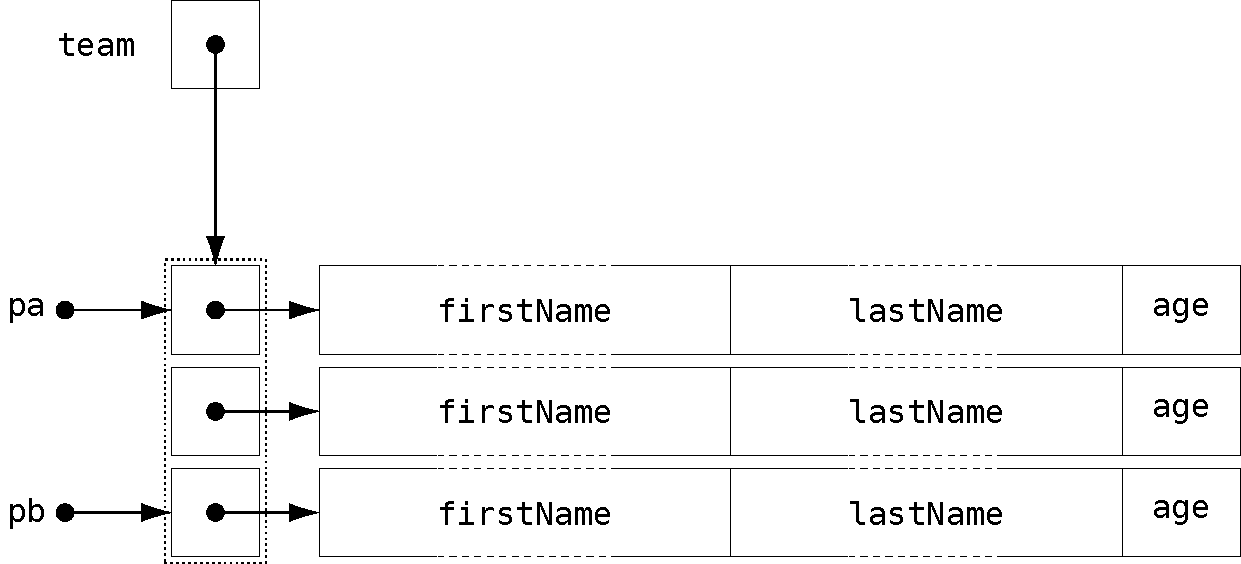
\includegraphics[scale=0.7]{images/sortPlayersCompareExample.pdf}
    \caption{Darstellung der beiden Pointer \mintinline{c}{pa} und
    \mintinline{c}{pb} auf jeweils ein Array-Element des
    \mintinline{c}{teams}-Array}
    \label{fig:sortPlayerCompareExample}
\end{figure}

Aus diesem Grund müssen wir diese Pointer als \mintinline{c}{Player**}
interpretieren, so dass wir durch eine Dereferenzierung einen Pointer auf ein
\mintinline{c}{Player}-Objekt erhalten:

\noindent\mintinline{c}{const Player *A = *(const Player**)pa;}

Sobald wir Pointer auf die beiden zu vergleichenden
\mintinline{c}{Player}-Objekte haben, können wir deren Nachnamen mittels der
\mintinline{c}{strcmp()}-Funktion lexikografisch vergleichen.

\begin{minted}{c}
int comparePlayerByLastName(const void *pa, const void *pb) {
    const Player *A = *(const Player**)pa;
    const Player *B = *(const Player**)pb;

    return strcmp(A->lastName, B->lastName);
}
\end{minted}

\section*{Funktion \texttt{freeTeam()}}

Die Funktion \mintinline{c}{freeTeam()} soll dazu dienen, den dynamisch
allokierten Speicher in geordneter Weise für ein ganzes Team wieder freizugeben.
Im Gegensatz zur Allokation des Speichers müssen wir jetzt in ungekehrter
Reihenfolge vorgehen, d.\,h. zuerst müssen wir den Speicher jedes einzelnen
\mintinline{c}{Player}-Objekts freigeben und im Anschluss den Speicher des
Arrays, in dem die Pointer auf die \mintinline{c}{Player}-Objekte abgelegt
wurden.

\begin{minted}{c}
void freeTeam(Player **team, int numPlayers) {
    for (int i = 0; i < numPlayers; i++) {
        free(team[i]);
    }
    free(team);
}
\end{minted}

Diese Reihenfolge muss eingehalten werden, denn hätten wir zuerst den Speicher
des Arrays freigegeben, hätten wir die Pointer auf die einzelnen
\mintinline{c}{Player}-Objekte verloren.
